\documentclass[11pt,a4paper]{report}
\usepackage[textwidth=37em,vmargin=30mm]{geometry}
\usepackage{calc,xunicode,amsmath,amssymb,paralist,enumitem,tabu,booktabs,datetime2,xeCJK,xeCJKfntef,listings}
\usepackage{tocloft,fancyhdr,tcolorbox,xcolor,graphicx,eso-pic,xltxtra,xelatexemoji}

\newcommand{\envyear}[0]{2025}
\newcommand{\envdatestr}[0]{2025-03-08}
\newcommand{\envfinaldir}[0]{webdb/2025/20250308/final}

\usepackage[hidelinks]{hyperref}
\hypersetup{
    colorlinks=false,
    pdfpagemode=FullScreen,
    pdftitle={Web Digest - \envdatestr}
}

\setlength{\cftbeforechapskip}{10pt}
\renewcommand{\cftchapfont}{\rmfamily\bfseries\large\raggedright}
\setlength{\cftbeforesecskip}{2pt}
\renewcommand{\cftsecfont}{\sffamily\small\raggedright}

\setdefaultleftmargin{2em}{2em}{1em}{1em}{1em}{1em}

\usepackage{xeCJK,xeCJKfntef}
\xeCJKsetup{PunctStyle=plain,RubberPunctSkip=false,CJKglue=\strut\hskip 0pt plus 0.1em minus 0.05em,CJKecglue=\strut\hskip 0.22em plus 0.2em}
\XeTeXlinebreaklocale "zh"
\XeTeXlinebreakskip = 0pt


\setmainfont{Brygada 1918}
\setromanfont{Brygada 1918}
\setsansfont{IBM Plex Sans}
\setmonofont{JetBrains Mono NL}
\setCJKmainfont{Noto Serif CJK SC}
\setCJKromanfont{Noto Serif CJK SC}
\setCJKsansfont{Noto Sans CJK SC}
\setCJKmonofont{Noto Sans CJK SC}

\setlength{\parindent}{0pt}
\setlength{\parskip}{8pt}
\linespread{1.15}

\lstset{
	basicstyle=\ttfamily\footnotesize,
	numbersep=5pt,
	backgroundcolor=\color{black!5},
	showspaces=false,
	showstringspaces=false,
	showtabs=false,
	tabsize=2,
	captionpos=b,
	breaklines=true,
	breakatwhitespace=true,
	breakautoindent=true,
	linewidth=\textwidth
}






\newcommand{\coverpic}[2]{
    % argv: itemurl, authorname
    Cover photo by #2~~(\href{#1}{#1})
}
\newcommand{\makeheader}[0]{
    \begin{titlepage}
        % \newgeometry{hmargin=15mm,tmargin=21mm,bmargin=12mm}
        \begin{center}
            
            \rmfamily\scshape
            \fontspec{BaskervilleF}
            \fontspec{Old Standard}
            \fontsize{59pt}{70pt}\selectfont
            WEB\hfill DIGEST
            
            \vfill
            % \vskip 30pt
            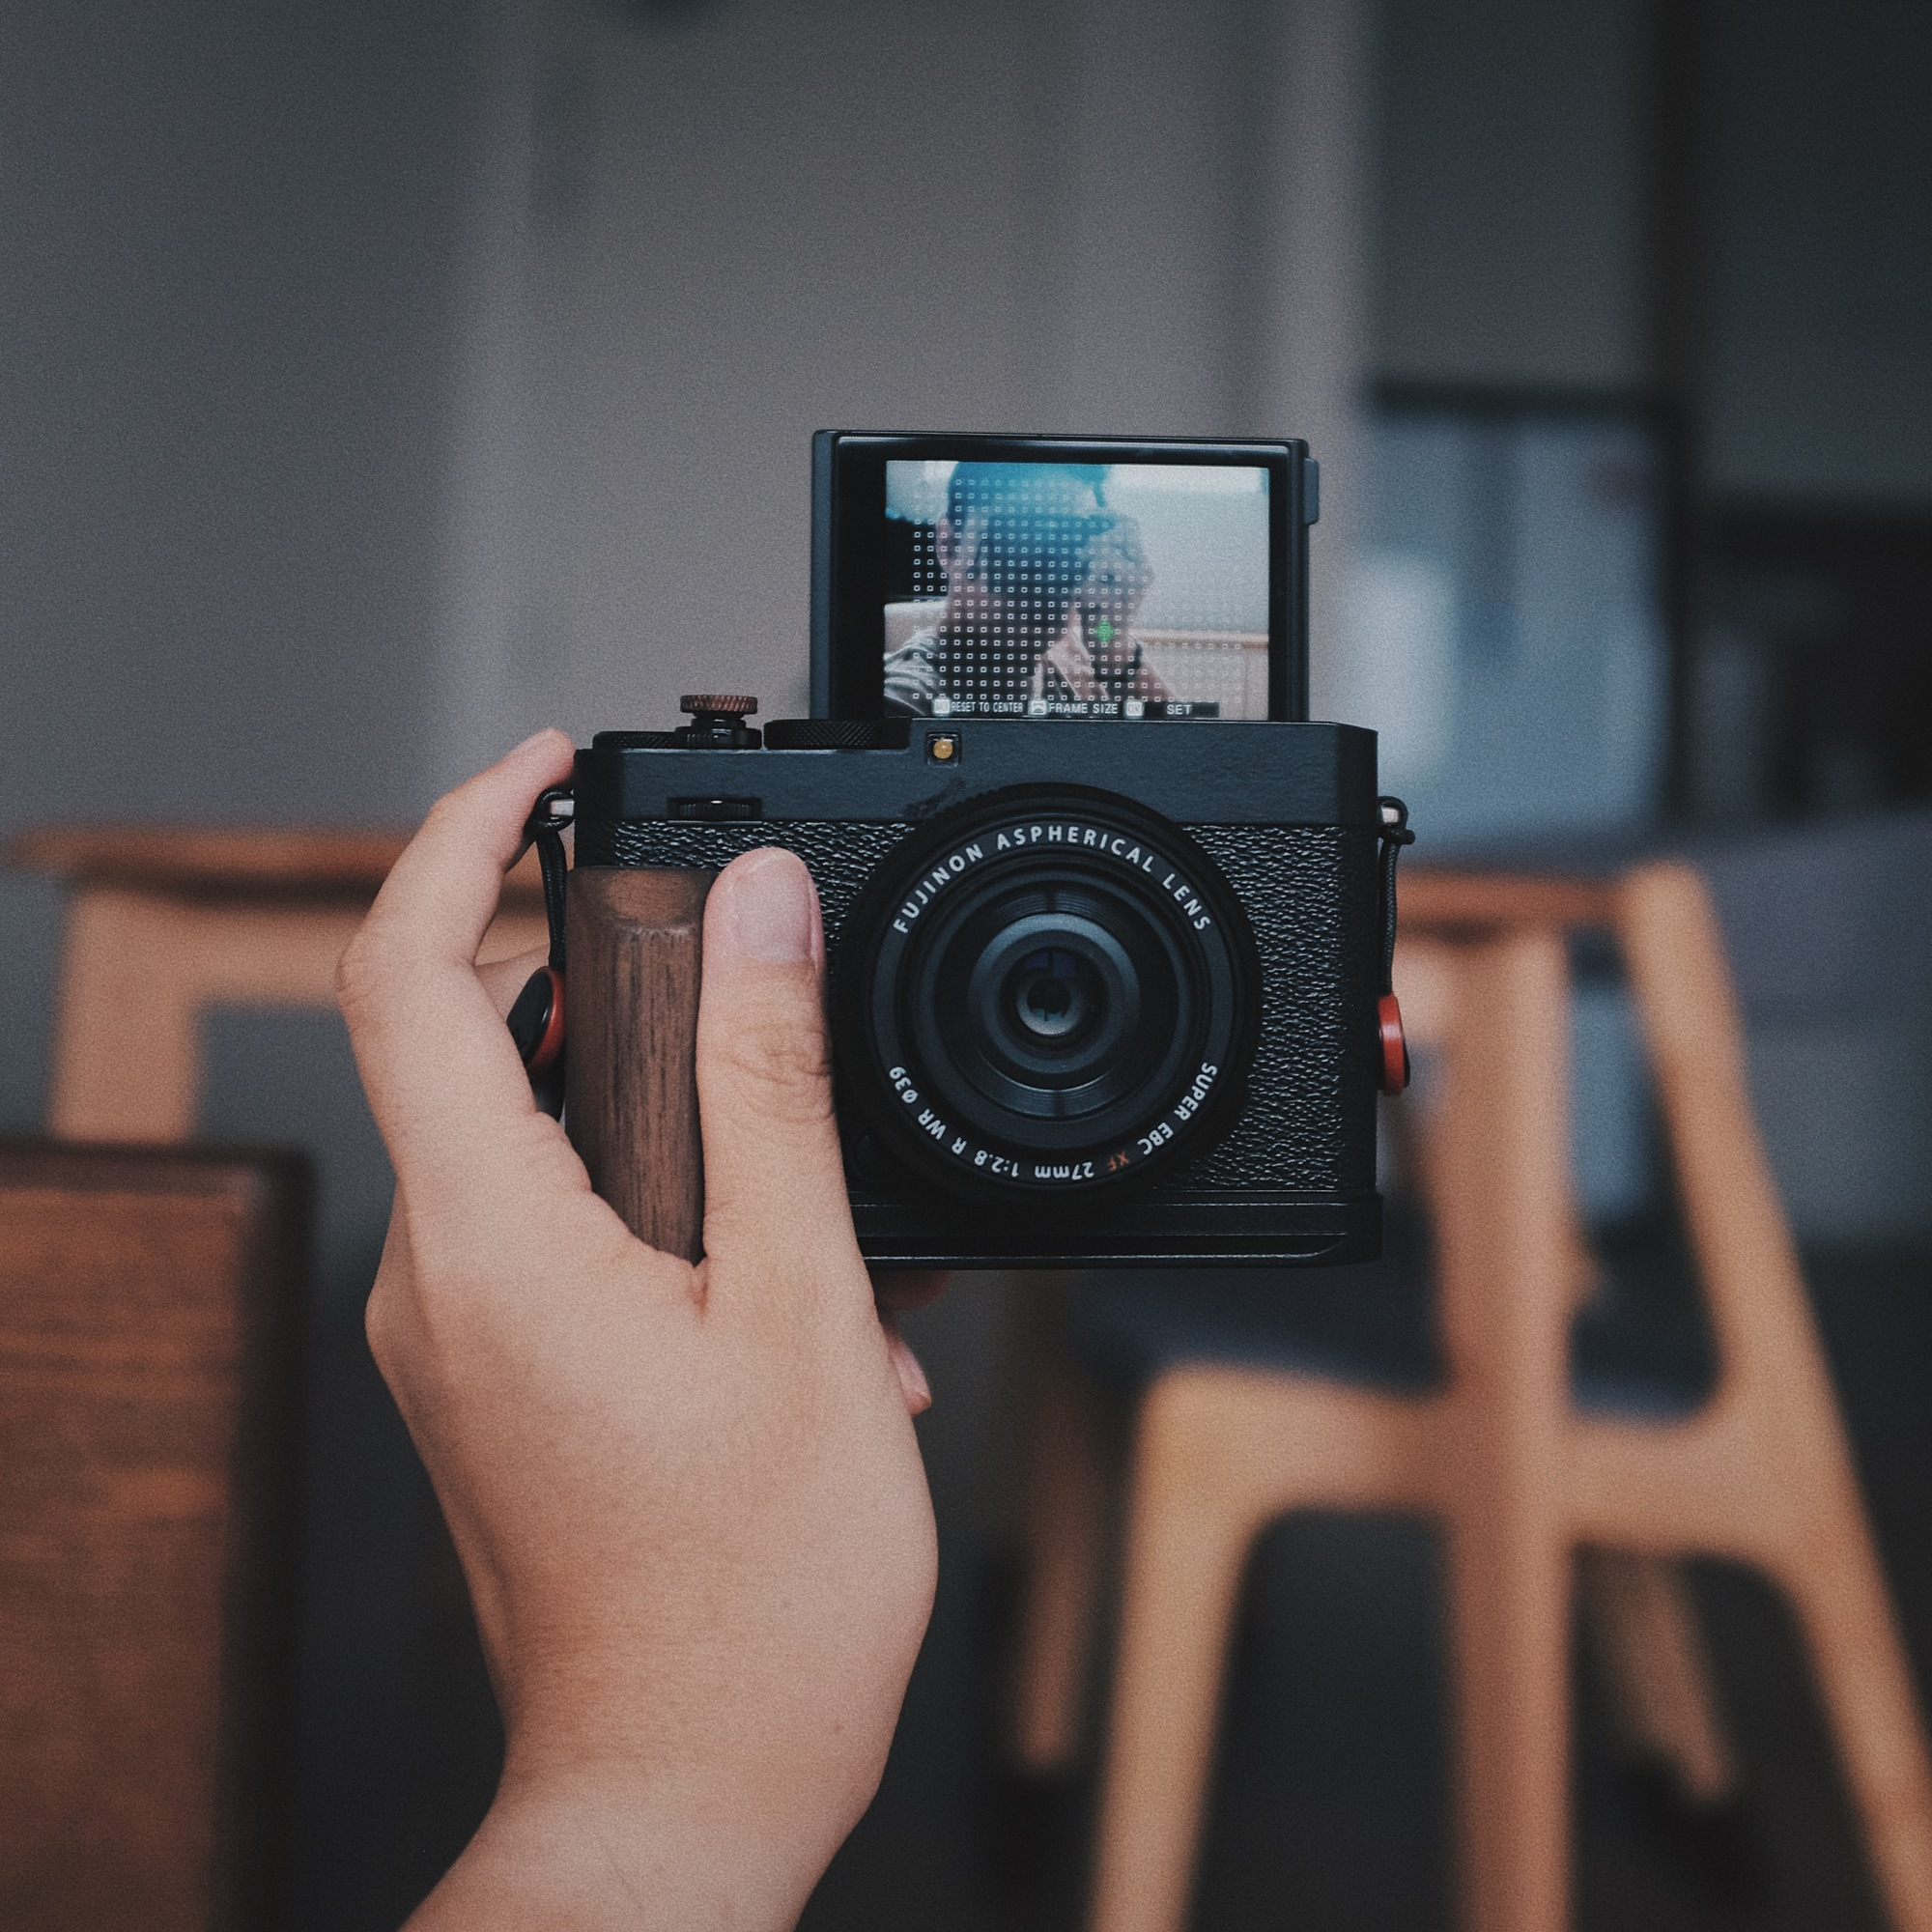
\includegraphics[width=\linewidth]{\envfinaldir/coverpic-prod.jpg}\par
            % \vskip 30pt
            \vfill

            \normalsize\rmfamily\scshape
            \copyright{} The Web Digest Project \hfill\large \envdatestr
        \end{center}
    \end{titlepage}
    % \restoregeometry
}
\newcommand{\simplehref}[1]{%
    \textcolor{blue!80!green}{\href{#1}{#1}}%
}
\renewcommand{\contentsname}{\center\Huge\sffamily\bfseries Contents\par\vskip 20pt}
\newcounter{ipartcounter}
\setcounter{ipartcounter}{0}
\newcommand{\ipart}[1]{
    % \vskip 20pt
    \clearpage
    \stepcounter{ipartcounter}
    \phantomsection
    \addcontentsline{toc}{chapter}{#1}
    % \begin{center}
    %     \Huge
    %     \sffamily\bfseries
    %     #1
    % \end{center}
    % \vskip 20pt plus 7pt
}
\newcounter{ichaptercounter}
\setcounter{ichaptercounter}{0}
\newcommand{\ichapter}[1]{
    % \vskip 20pt
    \clearpage
    \stepcounter{ichaptercounter}
    \phantomsection
    \addcontentsline{toc}{section}{\numberline{\arabic{ichaptercounter}}#1}
    \begin{center}
        \Huge
        \sffamily\bfseries
        #1
    \end{center}
    \vskip 20pt plus 7pt
}
\newcommand{\entrytitlefont}[1]{\subsection*{\raggedright\Large\sffamily\bfseries#1}}
\newcommand{\entryitemGeneric}[2]{
    % argv: title, url
    \parbox{\linewidth}{
        \entrytitlefont{#1}\par\vskip 5pt
        \footnotesize\ttfamily\mdseries
        \simplehref{#2}
    }\vskip 11pt plus 11pt minus 1pt
}
\newcommand{\entryitemGithub}[3]{
    % argv: title, url, desc
    \parbox{\linewidth}{
        \entrytitlefont{#1}\par\vskip 5pt
        \footnotesize\ttfamily\mdseries
        \simplehref{#2}\par\vskip 5pt
        \small\rmfamily\mdseries#3
    }\vskip 11pt plus 11pt minus 1pt
}
\newcommand{\entryitemAp}[3]{
    % argv: title, url, desc
    \parbox{\linewidth}{
        \entrytitlefont{#1}\par\vskip 5pt
        \footnotesize\ttfamily\mdseries
        \simplehref{#2}\par\vskip 5pt
        \small\rmfamily\mdseries#3
    }\vskip 11pt plus 11pt minus 1pt
}
\newcommand{\entryitemHackernews}[3]{
    % argv: title, hnurl, rawurl
    % \parbox{\linewidth}{
    %     \entrytitlefont{#1}\par\vskip 5pt
    %     \footnotesize\ttfamily\mdseries
    %     \simplehref{#3}\par
    %     \textcolor{black!50}{\href{#2}{#2}}
    % }\vskip 11pt plus 11pt minus 1pt
    \begin{minipage}{\linewidth}
            \entrytitlefont{#1}\par\vskip 5pt
            \footnotesize\ttfamily\mdseries
            \simplehref{#3}\par
            \textcolor{black!50}{\href{#2}{#2}}
    \end{minipage}\par\vskip 11pt plus 11pt minus 1pt
}







\begin{document}

\makeheader

\tableofcontents\clearpage




\ipart{Developers}
\ichapter{Hacker News}
\entryitemTwoLinks{Polars Cloud: The Distributed Cloud Architecture to Run Polars Anywhere}{https://news.ycombinator.com/item?id=43294566}{https://pola.rs/posts/polars-cloud-what-we-are-building/}

\entryitemTwoLinks{Europe's most wanted man plotted my murder and that of my colleague}{https://news.ycombinator.com/item?id=43293487}{https://theins.press/en/inv/279034}

\entryitemTwoLinks{Moscow-based global news network has infected Western AI tools}{https://news.ycombinator.com/item?id=43293121}{https://www.newsguardrealitycheck.com/p/a-well-funded-moscow-based-global}

\entryitemTwoLinks{Microsoft is plotting a future without OpenAI}{https://news.ycombinator.com/item?id=43292946}{https://techstartups.com/2025/03/07/microsoft-is-plotting-a-future-without-openai/}

\entryitemTwoLinks{Age Verification Laws: A Backdoor to Surveillance}{https://news.ycombinator.com/item?id=43292820}{https://www.eff.org/deeplinks/2025/03/first-porn-now-skin-cream-age-verification-bills-are-out-control}

\entryitemTwoLinks{AMD YOLO}{https://news.ycombinator.com/item?id=43292750}{https://geohot.github.io//blog/jekyll/update/2025/03/08/AMD-YOLO.html}

\entryitemTwoLinks{Athena spacecraft declared dead after toppling over on moon}{https://news.ycombinator.com/item?id=43292471}{https://www.theguardian.com/science/2025/mar/07/athena-spacecraft-mission-dead}

\entryitemTwoLinks{Introducing command And commandfor In HTML}{https://news.ycombinator.com/item?id=43292056}{https://developer.chrome.com/blog/command-and-commandfor}

\entryitemTwoLinks{Vtm: Text-Based Desktop Environment}{https://news.ycombinator.com/item?id=43291946}{https://github.com/directvt/vtm}

\entryitemTwoLinks{Ask HN: Do your eyes bug you even though your prescription is "correct"?}{https://news.ycombinator.com/item?id=43291922}{https://news.ycombinator.com/item?id=43291922}

\entryitemTwoLinks{Laser-based device can scan almost any sample of gas and tell you what's in it}{https://news.ycombinator.com/item?id=43291299}{https://phys.org/news/2025-02-laser-based-device-scan-sample.html}

\entryitemTwoLinks{Betting on the Pope was the original prediction market}{https://news.ycombinator.com/item?id=43290892}{https://nodumbideas.com/p/betting-on-the-pope-was-the-original}

\entryitemTwoLinks{Strobelight: A profiling service built on open source technology}{https://news.ycombinator.com/item?id=43290555}{https://engineering.fb.com/2025/01/21/production-engineering/strobelight-a-profiling-service-built-on-open-source-technology/}

\entryitemTwoLinks{Natural occurring molecule rivals Ozempic in weight loss, sidesteps side effects}{https://news.ycombinator.com/item?id=43289245}{https://medicalxpress.com/news/2025-03-naturally-molecule-rivals-ozempic-weight.html}

\entryitemTwoLinks{Matters Computational (2010) [pdf]}{https://news.ycombinator.com/item?id=43288861}{https://www.jjj.de/fxt/fxtbook.pdf}

\entryitemTwoLinks{Bye, Prime}{https://news.ycombinator.com/item?id=43288156}{https://www.tbray.org/ongoing/When/202x/2025/03/06/Canceled-Prime}

\entryitemTwoLinks{Ladder: Self-improving LLMs through recursive problem decomposition}{https://news.ycombinator.com/item?id=43287821}{https://arxiv.org/abs/2503.00735}

\entryitemTwoLinks{Rules to improve air quality are under attack}{https://news.ycombinator.com/item?id=43287563}{https://www.heatpumped.org/p/you-put-your-pitchfork-away-already}

\entryitemTwoLinks{Differentiable Logic Cellular Automata}{https://news.ycombinator.com/item?id=43286161}{https://google-research.github.io/self-organising-systems/difflogic-ca/?hn}

\entryitemTwoLinks{Why I find diffusion models interesting?}{https://news.ycombinator.com/item?id=43285726}{https://rnikhil.com/2025/03/06/diffusion-models-eval}\ichapter{Phoronix}
\entryitemGeneric{\hskip 0pt{}Wine 10.3 Wires Up Wayland Driver Clipboard Handling, Vulkan Video Decode Within WineD3D}{https://www.phoronix.com/news/Wine-10.3-Released}

\entryitemGeneric{\hskip 0pt{}GNOME 48 Release Candidate Brings Late Mutter Features \& Other Changes}{https://www.phoronix.com/news/GNOME-48-Release-Candidate}

\entryitemGeneric{\hskip 0pt{}Vulkan Video Continues Making Inroads, VP9 Decode Planned For This Year}{https://www.phoronix.com/news/Vulkan-Video-2025-Plans}

\entryitemGeneric{\hskip 0pt{}Ubuntu To Revert "-O3" Optimizations, Continues Quest For Easier ARM64 Installations}{https://www.phoronix.com/news/Ubuntu-No-O3-Easier-ARM64}

\entryitemGeneric{\hskip 0pt{}AMD Officially Confirms Ryzen 9 9900X3D + Ryzen 9 9950X3D Pricing \& Availability}{https://www.phoronix.com/news/Ryzen-9-9900X3D-9950X3D}

\entryitemGeneric{\hskip 0pt{}GCC 15 Now Enables AArch64 Early Scheduling For -O3/-Ofast Modes}{https://www.phoronix.com/news/GCC-15-AArch64-Early-Sched}

\entryitemGeneric{\hskip 0pt{}Unofficial ROCm SDK Builder Expanded To Support More GPUs}{https://www.phoronix.com/news/ROCm-SDK-Builder-6.1.2}

\entryitemGeneric{\hskip 0pt{}Intel Xe Driver Introducing SVM, EU Stall Sampling \& Other New Features For Linux 6.15}{https://www.phoronix.com/news/Intel-Xe-SVM-For-Linux-6.15}

\entryitemGeneric{\hskip 0pt{}New Round Of Driver Optimizations For AMD RadeonSI In Mesa 25.1}{https://www.phoronix.com/news/RadeonSI-New-Opts-Mesa-25.1}\ichapter{Dribbble}
\entryitemGeneric{\hskip 0pt{}Free Fly Apparel}{https://dribbble.com/shots/25727838-Free-Fly-Apparel}

\entryitemGeneric{\hskip 0pt{}Columbus Rapids® C-Wave}{https://dribbble.com/shots/25727535-Columbus-Rapids-C-Wave}

\entryitemGeneric{\hskip 0pt{}QLOUD - Logo Redesign}{https://dribbble.com/shots/25726630-QLOUD-Logo-Redesign}

\entryitemGeneric{\hskip 0pt{}Bloodhound Detective}{https://dribbble.com/shots/25726401-Bloodhound-Detective}

\entryitemGeneric{\hskip 0pt{}Logo Design for Streaming Platform (Unused for Sale)}{https://dribbble.com/shots/25726051-Logo-Design-for-Streaming-Platform-Unused-for-Sale}

\entryitemGeneric{\hskip 0pt{}Puzzle Fintech Website Design}{https://dribbble.com/shots/25651990-Puzzle-Fintech-Website-Design}

\entryitemGeneric{\hskip 0pt{}Dashboard for an Education Product ✦ Golf Pro}{https://dribbble.com/shots/25720487-Dashboard-for-an-Education-Product-Golf-Pro}

\entryitemGeneric{\hskip 0pt{}Proboscis Monkey}{https://dribbble.com/shots/25720978-Proboscis-Monkey}

\entryitemGeneric{\hskip 0pt{}Logofolio Update - March 2025}{https://dribbble.com/shots/25719985-Logofolio-Update-March-2025}

\entryitemGeneric{\hskip 0pt{}Bento grid barbershop platform UI}{https://dribbble.com/shots/25715947-Bento-grid-barbershop-platform-UI}

\entryitemGeneric{\hskip 0pt{}Cimet Slogan}{https://dribbble.com/shots/25710581-Cimet-Slogan}

\entryitemGeneric{\hskip 0pt{}FUUL // Branding Identity}{https://dribbble.com/shots/25719928-FUUL-Branding-Identity}

\entryitemGeneric{\hskip 0pt{}Real Estate Platform UI}{https://dribbble.com/shots/25711538-Real-Estate-Platform-UI}

\entryitemGeneric{\hskip 0pt{}Easy A Deck}{https://dribbble.com/shots/25715917-Easy-A-Deck}

\entryitemGeneric{\hskip 0pt{}Logistics Company Web Design Landing Page}{https://dribbble.com/shots/25708252-Logistics-Company-Web-Design-Landing-Page}

\entryitemGeneric{\hskip 0pt{}Letter C + Hummingbird}{https://dribbble.com/shots/25713900-Letter-C-Hummingbird}

\entryitemGeneric{\hskip 0pt{}Inner Truth}{https://dribbble.com/shots/25659901-Inner-Truth}

\entryitemGeneric{\hskip 0pt{}Landing Page: AI Testing}{https://dribbble.com/shots/25714074-Landing-Page-AI-Testing}

\entryitemGeneric{\hskip 0pt{}Star + Check Mark Icon Concept}{https://dribbble.com/shots/25709690-Star-Check-Mark-Icon-Concept}

\entryitemGeneric{\hskip 0pt{}FREELANCE (Finally)}{https://dribbble.com/shots/25710537-FREELANCE-Finally}

\entryitemGeneric{\hskip 0pt{}Recent Logo Designs - Jeroen van Eerden}{https://dribbble.com/shots/25709914-Recent-Logo-Designs-Jeroen-van-Eerden}

\entryitemGeneric{\hskip 0pt{}Wolf}{https://dribbble.com/shots/25707625-Wolf}

\entryitemGeneric{\hskip 0pt{}Boletus logo}{https://dribbble.com/shots/25709349-Boletus-logo}

\entryitemGeneric{\hskip 0pt{}Communication Illustration}{https://dribbble.com/shots/25700541-Communication-Illustration}


\ipart{Developers~~~~(zh-Hans)}
\ichapter{Solidot}
\entryitemGeneric{\hskip 0pt{}Google 以国家安全理由希望不被肢解}{https://www.solidot.org/story?sid=80730}

\entryitemGeneric{\hskip 0pt{}光首次被转化为超固体}{https://www.solidot.org/story?sid=80729}

\entryitemGeneric{\hskip 0pt{}NASA 关闭航海家的科学设备以节省电力}{https://www.solidot.org/story?sid=80728}

\entryitemGeneric{\hskip 0pt{}研究发现精液质量与男性寿命相关}{https://www.solidot.org/story?sid=80727}

\entryitemGeneric{\hskip 0pt{}NASA 首次在月球上使用 GPS }{https://www.solidot.org/story?sid=80726}

\entryitemGeneric{\hskip 0pt{}OpenAI 计划对博士水平的 AI 智能体收取 2 万美元月费}{https://www.solidot.org/story?sid=80725}

\entryitemGeneric{\hskip 0pt{}36 家石化巨头产生的碳排放占到了全球的一半}{https://www.solidot.org/story?sid=80724}

\entryitemGeneric{\hskip 0pt{}美国停止分享大使馆领事馆收集的空气质量数据}{https://www.solidot.org/story?sid=80723}

\entryitemGeneric{\hskip 0pt{}全球暖化威胁低纬度地区到粮食产量}{https://www.solidot.org/story?sid=80722}

\entryitemGeneric{\hskip 0pt{}犹他州要求美国应用商店验证用户年龄}{https://www.solidot.org/story?sid=80721}

\entryitemGeneric{\hskip 0pt{}2024 年图灵奖授予了奠定强化学习的计算机科学家 Andrew Barto 和 Richard Sutton}{https://www.solidot.org/story?sid=80720}

\entryitemGeneric{\hskip 0pt{}苹果对英国的后门命令提起上诉}{https://www.solidot.org/story?sid=80719}

\entryitemGeneric{\hskip 0pt{}科学家创造猛犸鼠}{https://www.solidot.org/story?sid=80718}

\entryitemGeneric{\hskip 0pt{}TCL 在高端电视机出货量上超过 LG 仅次于三星}{https://www.solidot.org/story?sid=80717}

\entryitemGeneric{\hskip 0pt{}宇宙最早的水可能形成于大爆炸后的 1-2 亿年}{https://www.solidot.org/story?sid=80716}

\entryitemGeneric{\hskip 0pt{}韦伯望远镜发现有复杂大气层的流浪行星}{https://www.solidot.org/story?sid=80715}

\entryitemGeneric{\hskip 0pt{}兄弟打印机通过强制性更新固件禁用第三方墨盒}{https://www.solidot.org/story?sid=80714}

\entryitemGeneric{\hskip 0pt{}Homebrew Computer Club 成立 50 周年}{https://www.solidot.org/story?sid=80713}

\entryitemGeneric{\hskip 0pt{}Firefox 136 释出,支持垂直标签}{https://www.solidot.org/story?sid=80712}\ichapter{V2EX}
\entryitemGeneric{\hskip 0pt{}[分享发现] 通过 Moj Telekom 获取一年 perplexty ai pro 的会员}{https://www.v2ex.com/t/1116802}

\entryitemGeneric{\hskip 0pt{}[程序员] 轻松升级 JS 混淆 反 AI 分析破解}{https://www.v2ex.com/t/1116801}

\entryitemGeneric{\hskip 0pt{}[问与答] AI+低代码平台 是否有市场?}{https://www.v2ex.com/t/1116800}

\entryitemGeneric{\hskip 0pt{}[程序员] 关于 winui3 本地化功能的一些看法,欢迎讨论}{https://www.v2ex.com/t/1116798}

\entryitemGeneric{\hskip 0pt{}[投资] 交易经验不到 2 年,需要开创业科创,人情社会,有没有方案}{https://www.v2ex.com/t/1116797}

\entryitemGeneric{\hskip 0pt{}[加密货币] 2025 年人民币购买 USDT 比较好的方式有哪些?}{https://www.v2ex.com/t/1116796}

\entryitemGeneric{\hskip 0pt{}[分享创造] [旅行 APP 产品诞生日记] 9day/100days}{https://www.v2ex.com/t/1116795}

\entryitemGeneric{\hskip 0pt{}[问与答] 请问 https://1.0.0.1/dns-query 有好用靠谱的平替吗?}{https://www.v2ex.com/t/1116794}

\entryitemGeneric{\hskip 0pt{}[问与答] 美国亚马逊一直联系不上客服,提示错误}{https://www.v2ex.com/t/1116793}

\entryitemGeneric{\hskip 0pt{}[iOS] 求推荐 2025 年 ios/ipados/mac 的视频播放器}{https://www.v2ex.com/t/1116792}

\entryitemGeneric{\hskip 0pt{}[Apple] 2025 年 TCL Q10K+ APPLE TV 无 NAS 体验}{https://www.v2ex.com/t/1116791}

\entryitemGeneric{\hskip 0pt{}[职场话题] 下个工作是继续前端还是前端偏全栈}{https://www.v2ex.com/t/1116790}

\entryitemGeneric{\hskip 0pt{}[分享发现] 《I Want to Love You Till Your Dying Day》(きみが死ぬまで恋をしたい)粉丝资讯站}{https://www.v2ex.com/t/1116789}

\entryitemGeneric{\hskip 0pt{}[分享创造] 很快啊,让 AI 写了一个一键下载当前网页的封面图(OG)浏览器插件,域名也很牛逼(ogimage.download)}{https://www.v2ex.com/t/1116787}

\entryitemGeneric{\hskip 0pt{}[硬件] 实测惠普雷电 4 扩展坞 G4 (HP thunderbolt g4) 支持 4.5K (5120 x 2160) 输出}{https://www.v2ex.com/t/1116786}

\entryitemGeneric{\hskip 0pt{}[问与答] 5ber 跑路,老用户怎么办}{https://www.v2ex.com/t/1116785}

\entryitemGeneric{\hskip 0pt{}[宽带症候群] 坐标上海,触发运营商风控被直接断网}{https://www.v2ex.com/t/1116784}

\entryitemGeneric{\hskip 0pt{}[Apple] Apple Watch 可以忽略户外骑车的自动监测吗?}{https://www.v2ex.com/t/1116783}

\entryitemGeneric{\hskip 0pt{}[问与答] 求一款手机当热点机,要求,开热点能开一天(或半天?)不重,便宜, 5G(信号要好),其他无所谓}{https://www.v2ex.com/t/1116782}

\entryitemGeneric{\hskip 0pt{}[问与答] Mac 上运行 cursor 总是无法连上 ssh host}{https://www.v2ex.com/t/1116781}

\entryitemGeneric{\hskip 0pt{}[问与答] 想发帖,突然出现了莫名其妙的东西}{https://www.v2ex.com/t/1116779}

\entryitemGeneric{\hskip 0pt{}[浏览器] 关于 V 友 @Notamo 对 Alook 浏览器 iOS 版本刷好评质疑的回复}{https://www.v2ex.com/t/1116778}

\entryitemGeneric{\hskip 0pt{}[OpenAI] 现阶段 cursor 中可以稳定调用 claude 3.7 吗? poe.com 中的 claude 3.7 ,是被降智的吗?这两个平台,哪个更好?}{https://www.v2ex.com/t/1116777}

\entryitemGeneric{\hskip 0pt{}[NAS] 今天突然断电,然后铁威马 D2-310 就无法开机亮灯了,有没有靠谱的维修?}{https://www.v2ex.com/t/1116775}

\entryitemGeneric{\hskip 0pt{}[OpenAI] bybit 虚拟卡给 Claude api 充值}{https://www.v2ex.com/t/1116772}

\entryitemGeneric{\hskip 0pt{}[分享创造] 阿里巴巴开源 Wan 2.1 强大的视频模型,做了一个体验平台}{https://www.v2ex.com/t/1116771}

\entryitemGeneric{\hskip 0pt{}[问与答] 求推荐可以记录一天中各个任务耗时的工具}{https://www.v2ex.com/t/1116770}

\entryitemGeneric{\hskip 0pt{}[VPS] Bandwagon NODESEEK-BIGGERBOX 融合怪+AFF 购买地址。}{https://www.v2ex.com/t/1116769}

\entryitemGeneric{\hskip 0pt{}[Android] 有没有开源硬件,开源安卓设备?}{https://www.v2ex.com/t/1116768}

\entryitemGeneric{\hskip 0pt{}[职场话题] 有朋友想入灰产,该如何说服他}{https://www.v2ex.com/t/1116767}

\entryitemGeneric{\hskip 0pt{}[问与答] 大家买过 80\%减霜的冰柜嘛?效果如何?}{https://www.v2ex.com/t/1116766}

\entryitemGeneric{\hskip 0pt{}[分享发现] Notion Mail 已拿到}{https://www.v2ex.com/t/1116765}

\entryitemGeneric{\hskip 0pt{}[分享发现] 2025 了 信息差生意依然能赚钱}{https://www.v2ex.com/t/1116763}

\entryitemGeneric{\hskip 0pt{}[汽车] 小米最近各路媒体推太多了 感觉有点烦了}{https://www.v2ex.com/t/1116762}

\entryitemGeneric{\hskip 0pt{}[Apple] 入手了日版苹果 16,没想到苹果 ai 的这个功能在大陆无论如何都是用不了了的}{https://www.v2ex.com/t/1116760}

\entryitemGeneric{\hskip 0pt{}[问与答] cloudflare 的统计分析就是假数据是么?}{https://www.v2ex.com/t/1116759}

\entryitemGeneric{\hskip 0pt{}[职场话题] 一年换一家公司,但完全没有个人原因,这个对于求职有多大影响,如何说明?}{https://www.v2ex.com/t/1116758}

\entryitemGeneric{\hskip 0pt{}[问与答] macOS 15 现在稳定了么,各位使用过程还有遇到什么恶性 bug 吗?}{https://www.v2ex.com/t/1116757}

\entryitemGeneric{\hskip 0pt{}[问与答] 大家生产环境都用什么虚拟化解决方案呢?}{https://www.v2ex.com/t/1116756}

\entryitemGeneric{\hskip 0pt{}[职场话题] 失业了,副业也不行,咋整}{https://www.v2ex.com/t/1116754}

\entryitemGeneric{\hskip 0pt{}[macOS] 救救孩子之 macos 15 又发疯了}{https://www.v2ex.com/t/1116753}

\entryitemGeneric{\hskip 0pt{}[问与答] 需要长时间盯屏幕应该如何配眼镜?}{https://www.v2ex.com/t/1116752}

\entryitemGeneric{\hskip 0pt{}[问与答] Win11 鼠标 左键 单击 经常会 出现 双击 左键的效果, 有 v 友遇到过吗?}{https://www.v2ex.com/t/1116751}

\entryitemGeneric{\hskip 0pt{}[分享创造] xsAI - 包体积小于 6KB 的 Vercel AI SDK 平替}{https://www.v2ex.com/t/1116750}

\entryitemGeneric{\hskip 0pt{}[问与答] IOS 下 deepseek 登陆问题}{https://www.v2ex.com/t/1116747}

\entryitemGeneric{\hskip 0pt{}[分享发现] 使用 git svn 进行版本控制(本地使用 git 仓库,远程使用使用 svn 仓库)}{https://www.v2ex.com/t/1116746}

\entryitemGeneric{\hskip 0pt{}[Arc] Arc 关闭 Tab 后,内存没有及时释放。}{https://www.v2ex.com/t/1116745}

\entryitemGeneric{\hskip 0pt{}[问与答] 当下一加 Ace 中端机还有支持好的 ROM 可以刷吗?}{https://www.v2ex.com/t/1116744}

\entryitemGeneric{\hskip 0pt{}[问与答] 有对日本香了解的吗,想入伽罗桃山,为什么闲鱼和淘宝差价那么大?闲鱼清一色 60 上下横跳,淘宝全都 1K+?}{https://www.v2ex.com/t/1116742}

\entryitemGeneric{\hskip 0pt{}[生活] 2023 年个税被秋后了}{https://www.v2ex.com/t/1116741}


\ipart{Generic News}







\clearpage
\leavevmode\vfill
\footnotesize

Copyright \copyright{} 2023-2025 Neruthes and other contributors.

This document is published with CC BY-NC-ND 4.0 license.

The entries listed in this newsletter may be copyrighted by their respective creators.

This newsletter is generated by the Web Digest project.

The newsletters are also delivered via Telegram channel \CJKunderline{\href{https://t.me/webdigestchannel}{https://t.me/webdigestchannel}}.\\
RSS feed is available at \CJKunderline{\href{https://webdigest.pages.dev/rss.xml}{https://webdigest.pages.dev/rss.xml}}.

This newsletter is available in PDF at
\CJKunderline{\href{https://webdigest.pages.dev/}{https://webdigest.pages.dev/}}.

The source code being used to generate this newsletter is available at\\
\CJKunderline{\href{https://github.com/neruthes/webdigest}{https://github.com/neruthes/webdigest}}.

This newsletter is also available in
\CJKunderline{\href{http://webdigest.pages.dev/readhtml/\envyear/WebDigest-20250308.html}{HTML}} and
\CJKunderline{\href{https://github.com/neruthes/webdigest/blob/master/markdown/\envyear/WebDigest-20250308.md}{Markdown}}.


\coverpic{https://unsplash.com/photos/CLlL393ykrY}{The New York Public Library}


\end{document}
